\section{The DOM Firewall}

We now present the DOM Firewall's components and how they interact with each other. First, we give a overview of current defence solutions and how they into our model. Further details of these different approaches are described in Section 5.

\subsection{Web application architecture}
Figure~\ref{fig:web_architecture} shows a typical architecture for web applications. There are several different places where vulnerability defences can be integrated. We give a brief description of what can be done at each point:
\begin{itemize}
	\item  At the application layer, the developer is trying to defend itself against malicious users. The first line of defence for these vulnerabilities lies in the application logic itself. The developer might choose to ensure safety of the code, either by use existing solutions, or by securing the code themselves, for example, by applying static analysis to detect unsanitised input.
	\item The information then goes through the server-side networking of the web application. At this point, defences include generic firewalls and more specific Web Application firewalls (WAFs), which defend against  attacks such as DDoS, SQL injections and XSS.
	\item At the client side layer, there is another networking component. At this point, the user is defending from malicious websites, and may have their own generic firewall, blacklisted websites, and proxies. 
	\item Finally, the information gets to the user's browser. This will usually have built-in defences, such as Chrome's XSS auditor. The user might also install browser-dependent functionality, such as extensions like NoScript.
\end{itemize}

It should be noted that many of these approaches are either too specific or too generic. For example, a WAF might be enough to defend against most XSS attacks, but it would require each individual developer to have the necessary knowledge and resources to integrate one. A proxy at the client-side will usually have a generic set of rules to apply on incoming network traffic, and this will often lead to an elevated rate of false positives. Browser built-in defences are very coarse, and will only work on a subset of exploits. Chrome's XSS auditor, for example, only attempts to defend against reflected XSS. 

Our approach, instead, focuses on application-specific detection at the client-side layer, and thus, doesn't rely on any server-side infrastructure and is more accurate than many client-side solutions. Furthermore, it is complementary to the aforementioned techniques: a WAF will not reduce the security of our approach by any means, and having these two work in tandem is beneficial to the user's experience. On the other hand, an user that has not installed our extension will receive none of the benefit.
\begin{figure}[h]
	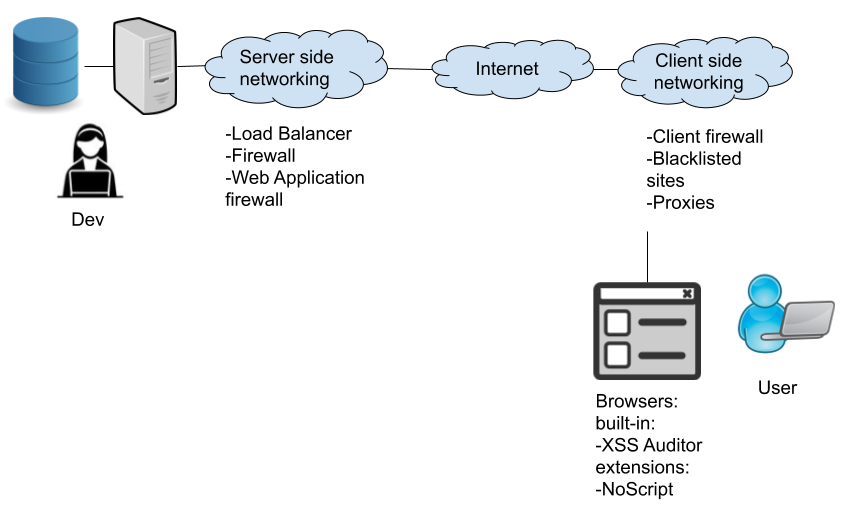
\includegraphics[scale=0.3]{img/web_architecture.png}
	\caption{Architecture of typical web applications. Different security solutions apply at distinct layers.}
	\label{fig:web_architecture}
\end{figure}


\subsection{Client-side Approach}
 Commonly, bug bounty hunters and penetration testers will scour websites to find vulnerabilities and alert developers of issues in these, as well as potential fixes. Developers will then fix the bugs accordingly so that users are not subject to vulnerabilities. Inspired by this workflow, we believe this process can be partly automated using a firewall-based approach, so that users don't have to wait for developers to update their code. Figure~\ref{fig:dom_firewall} illustrates how the firewall can be used to guarantee full client-side protection: A user loads a request, such as www.myblog.com, this request might come back with malicious code in the form of an XSS attack. Before rendering the webpage in the browser, an extension can analyze the potentially malicious document, doing so by loading signatures which a developer (a bug bounty hunter, for example) has uploaded to a database, and completely eliminating the injected code. Finally, the extension returns a clean HTML document, which the browser then proceeds to render.
 
 \begin{figure}[h]
 	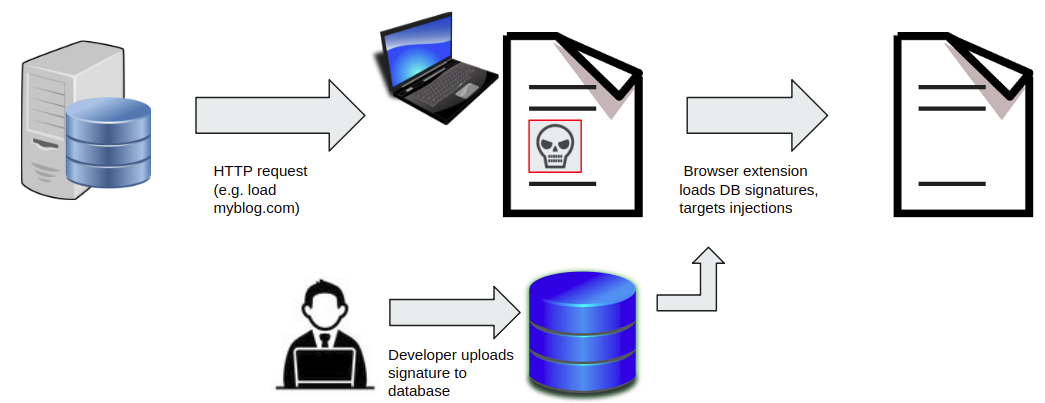
\includegraphics[scale=0.23]{img/dom_firewall.png}
 	\caption{The DOM Firewall approach for protection against XSS.}
 	\label{fig:dom_firewall}
 \end{figure}

In order to further illustrate this approach, we present a small example of how DOM context can be used to defend against XSS (this is reproducible in an off-the-box WordPress installation running the Responsive Cookie Consent plugin, v1.8, Chrome's XSS auditor, for example, does not protect against this). Consider a website running PHP on the backend that takes user input and stores it to later display it to another user, in this case, the value 'border-size'.
\\
\begin{lstlisting}
<div class="rcc-panel group" 
border-bottom:<@\textcolor{red}{<?php rcc\_value('border-size')};>
\end{lstlisting}
This div element will display the border-bottom attribute that was input by the user, under normal circumstances, it might display something such as: 
\begin{lstlisting}
<div class="rcc-panel group" 
border-bottom: <@\textcolor{red}{0px solid rgb(85,85,85)}@>;>
\end{lstlisting}
However, if the user is malicious, it could inject a script through the border-size variable, as it is not sanitized on the server side. If we have
\begin{lstlisting}
border-size = ""><script>alert('XSS')</script>
\end{lstlisting}
then, the browser will render the following, executing the injected script:
\begin{lstlisting}
<div class="rcc-panel group" 
border-bottom:<@\textcolor{red}{"">
<script>alert('XSS')</script>}
\end{lstlisting}

Assuming an analyst has knowledge of how the full HTML should render without any injections, they can single out the point of injection, by separating user input from the server-side template, and get rid of the malicious script entirely. This works by essentially "sandwiching" the injection point. In the example, the injected script in red can be easily distinguished from the rest of the HTML template by looking for the div element that comes right before it from the top of the document, and the element that comes right after it from the bottom. TODO: mention why this might not work for some pages later on.

In the following sections we give a detailed description of each component of our system, the challenges that arise when trying to defend against XSS client-side, and the tools provided by the browser to facilitate our methods. 
 
 \subsection{Firewall Signatures}
	 The firewall signatures are at the core of our defense strategy. These must be precise enough for the extension to single out the intended injection, and not an otherwise vital element of the website. Since we are only relying on DOM knowledge, these signatures must be related to HTML features, for example, specifying elements and element attributes that are unique to where the exploit might occur. The basis for our signatures relies on two observations: first, an injection has a start and end point, that is, an element can only be injected between a specific HTML node and its immediate sibling in the HTML tree; second, in a well-formed DOM, the injected element will not be able to change its location without any JavaScript execution. Thus, our basic approach at signature definition is to specify an injection's start and it's end, and the extension will stop any JavaScript from executing in this section of the HTML. Of course, it's up to the signature developer to decide whether there should be any JavaScript executing in this location. However, it is often easy to make this decision, as there are many input parameters which clearly shouldn't execute any JavaScript.
	 
	An immediate concern that can come up is who writes these signatures. We believe CVEs to be an ideal source for these: as discussed previously, bug bounty hunters and penetration testers will commonly identify issues in application code, inform developers and publish it for the benefit of the community in the form of CVEs. Our system adds an extra component to this workflow, where hackers and security enthusiasts also write the signatures to defend users.
 
 \subsection{Firewall Signature Language}
 Our signature language needs to be such that it has enough power of expression for the developer to be as precise as they need. Due to the nature of our signature definitions, a regex language should suffice to express precise sections of the HTML. Furthermore, a regex language allows us to identify malformed HTML before it renders on the browser, as described below.
 
 \subsection{Firefox Extension}
 The extension model provided by several browsers allows us to interpose on any functionality of a website in a privileged execution environment, unavailable to any third-party. Firefox in particular allows the interception of any script elements in the HTML, via the \textbf{beforescriptexecute} event. Thus, whenever any malicious script wants to run, we can first audit it and determine whether it should execute or not, according to rules defined by the firewall. While not all XSS is triggered by script elements, they do require JavaScript. Thus, we can modify any event listeners as well, effectively interposing on any JavaScript execution. Any required modifications of the HTML can be done in-place, as the website loads. 
 
We have assumed that we know how the HTML will be rendered on the client-side, but even with this knowledge, there are injections which might alter the expected placement of different elements. For example, a <tr> element may only have direct children <th> or <td>. In our experiments, we found that an injection occurring as a direct child of the <tr> might cause the injected element to be rendered above the <tr> in the DOM. This defies one of our key observations with regards to injection placements. Therefore, we can't wait until the website is rendered client-side to start interposing on code execution. To account for this, we make use of the webRequest API provided by Firefox to filter incoming responses, tagging all elements with special identifiers, allowing us to have a similar representation of the HTML as the signature developer had in mind. This technique is susceptible to a knowledgeable attacker, who can identify all attributes of the starting and end points of the injection sections, to trick our extension into thinking that the section is already over by injecting a duplicate of the end node. To combat this, we use a top-down, bottom-up approach when looking for attacks. Our main observation in this case is that the injected code cannot be infinitely long. Thus, the real end node will eventually follow the injection, and we can backtrack the HTML tree from the end of the document to find it. Thus, an attacker cannot trick the extension into analysing a smaller section of the document.
